\setlength{\footskip}{8mm}

\chapter{Clustering Human Behaviors with Dynamic Time 
Warping and Hidden Markov Models}
\label{ch:clustering}

\textit{In this chapter, we propose and experimentally evaluate a new 
method for clustering human behaviors that is suitable for
bootstrapping an anomaly detection module for intelligent video
surveillance systems. The method uses dynamic time warping,
agglomerative hierarchical clustering, and hidden Markov models to
provide an initial partitioning of a set of observation sequences then
automatically identifies where to cut off the hierarchical clustering
dendrogram. We show that the method is extremely effective, providing
100\% accuracy in separating anomalous from typical behaviors on
real-world testbed video surveillance data.}

\section{Introduction}
\label{sec:clustering-intro}

Human behavior understanding is an important component of a wide
variety of desirable intelligent systems.  However, the problem is
very difficult, due to the wide range of activities possible in any
given context and the large amount of variability within any
particular activity. Many researchers have attempted to build systems
able to interpret and understand human behaviors. The most classic
work is from \shortciteA{yamato92hmm}, who model
tennis actions using hidden Markov models (HMMs). 
\shortciteA{du06activity} present an approach to recognize
interaction activities using dynamic Bayesian networks (DBNs) that
outperforms conventional HMMs. \shortciteA{gao04dining}
use a single mixture-of-Gaussian HMM, in which the states represent
the stages of dining activities, to monitor the eating behavior of
elderly people in a nursing home.

As video monitoring is becoming more ubiquitous in our lives, research
on advanced video surveillance analysis is increasingly important.  To
help security personnel work reliably and efficiently, we would like
to filter out typical events, and in cases of anomalous events,
automatically raise an alarm or present the event to a human operator
for consideration as a security threat. Most existing work assumes
that the number of ``normal'' behavior patterns need to be known
beforehand. For example, \shortciteA{nair02surveillance} built an
automated video surveillance system using HMMs, each modeling a
common, predefined activity in a scene.

In more recent years, research has started to focus on unsupervised
analysis and clustering of behaviors in a particular scene for a
variety of purposes including anomaly detection, surveillance, and
classification. \shortciteA{zhong04detection} treat video segments as
documents and cluster the documents based on the co-occurrence
information. \shortciteA{li06behavior} cluster human gestures by
constructing an affinity matrix using dynamic time warping (DTW;
Sakoe, 1978)\nocite{sakoe78dtw} then apply the normalized-cut approach
to cluster the gestures. \shortciteA{hautamaki08clustering} apply DTW
and use the pairwise DTW distances as input to a hierarchical
clustering process in which $k$-means is used to fine-tune the output.

Here we use a combination of clustering and HMMs to group
human behaviors in a scene. There is some recent related work using
graphical models such as HMMs to cluster behavior
patterns. \shortciteA{li99pattern} use the Bayesian information
criterion (BIC) for HMM model selection and construct a binary
hierarchical clustering dendrogram to initialize data partitions based
on a sequence-to-model likelihood distance measure. They then compare
each pair of clusters using a partition mutual information (PMI)
criterion \shortcite{bahl86speech} to find the optimal number of
clusters.

\shortciteA{xiang05profiling} model the distribution of
activity data in a scene using a Gaussian mixture model (GMM) and also
employ the BIC to select the optimal number of behavior classes prior
to HMM training.

\shortciteA{swears08clustering} propose hierarchical HMM-based clustering
to find and cluster motion trajectories and velocities in a highway
interchange scene. They build up a set of HMMs incrementally. For each
new trajectory, they first test the likelihood of the trajectory
according to each existing HMM model.  If the new observation is not
fit by any existing model, it is considered deviant and is grouped
with other deviant observations to form a new HMM.

\shortciteA{alon03clustering} propose a method to discover groupings of
similar object motions. They apply a finite mixture of HMMs where the
number of mixture components is assumed to be known. They estimate the
number of clusters using the minimum description length (MDL)
criterion \shortcite{rissanen98mdl}, a penalized likelihood measure.

In this dissertation, we propose a new method for clustering human
behaviors in the context of video surveillance.  After extracting
sequences of features representing individual human behaviors in a
given scene, we use DTW to measure the pairwise similarity between
sequences. Then we construct an agglomerative hierarchical clustering
dendrogram based on the DTW similarity measure. To find the optimal
set of behavior clusters, we start at the root of the tree, train a
HMM on the patterns in that cluster, and determine how well the HMM
models the set of patterns in the cluster.  When we find that a HMM is
an insufficient representation of the patterns in a given cluster, we
throw away that HMM and recursively consider each of the child
clusters according to the pre-calculated DTW-based dendrogram. Our
method is able to automatically find the common human behaviors
occurring in a given scene. In an experiment with a testbed video
surveillance data set, we find that the method separates typical
behaviors and abnormal behaviors into separate sets of clusters with
100\% accuracy.

The most similar related work is that
of \shortciteA{oates01clustering}, who first proposed the idea of
using the DTW with HMMs to cluster time series. They use the DTW
dendrogram cut off at an arbitrary depth as an initial partition of
the training sequences, then they train HMMs on each partition
iteratively until they have a set of HMMs that models all of the
training sequences.  They apply their method to simulated time series
with good results but report obtaining poor clustering results in an
experiment with real robot sensor data.

As we shall see in later chapters, the method improves upon the state
of the art in intelligent video surveillance applications by
bootstrapping human behavior classification and anomaly detection
modules in a given installation. Once a set of initial clusters and
corresponding HMMs representing typical behavior is determined, we can
easily find which cluster a new sequence should fall into by
performing statistical tests on the sequence's likelihood according to
each HMM model.  When the likelihood is low according to all of the
pre-existing clusters, we can consider the sequence to be anomalous
and alert a human operator. When the likelihood is sufficiently high
for one of the pre-existing models, we can simply incrementally update
the sufficient statistics for that model.  This approach would allow
raising alerts for behaviors inconsistent with the
automatically-derived typical behavior profile for the scene while
providing adaptation to gradual changes in typical behavior patterns
over time. We do not focus on these incremental learning and anomaly
detection issues in this chapter. We consider these issues in later
chapters.

In the rest of this chapter, I provide the details of our human
behavior clustering algorithm in
Section \ref{sec:clustering-algorithm}, demonstrate the feasibility of
the algorithm with an experimental evaluation in
Section \ref{sec:clustering-results}, and then conclude and point to
future work in Section \ref{sec:clustering-discussion}.

\section{Human Behavior Pattern Clustering}
\label{sec:clustering-algorithm}

\subsection{Overview}

\begin{figure}[t]
  \centering
  \subfloat[]{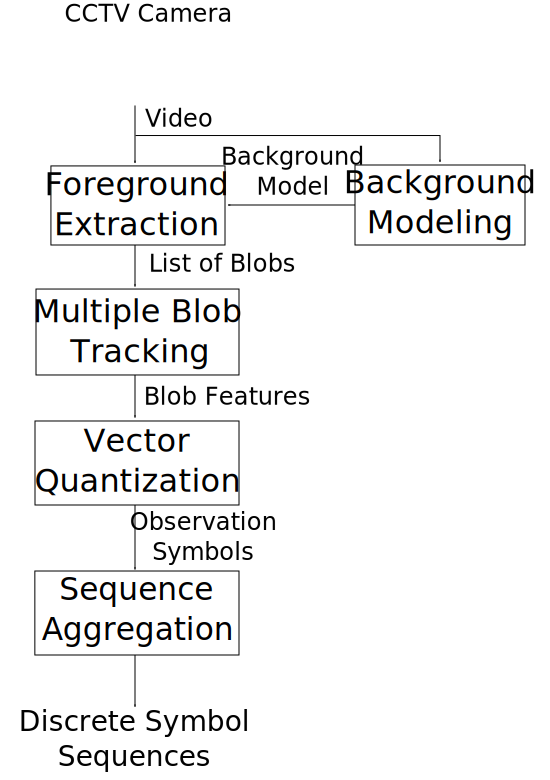
\includegraphics[scale=0.4]{figures/blob-extraction-block-diagram}
  \label{fig:overview-blob}}
  \subfloat[]{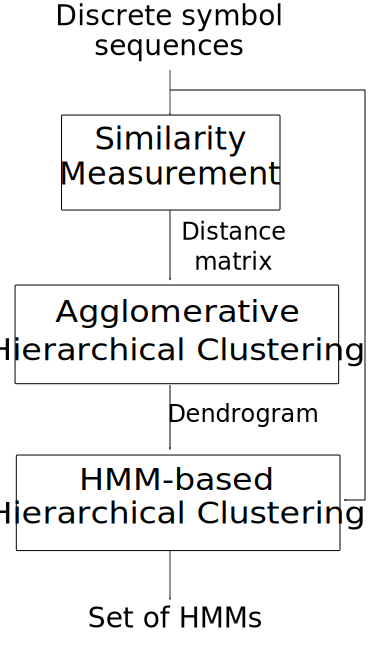
\includegraphics[scale=0.4]{figures/behavior-clustering-block-diagram}
  \label{fig:overview-clustering}}
  \caption[Block diagrams for the proposed method.]{\small Block
    diagrams for the proposed method.  (a) Blob extraction flow. (b)
    Behavior clustering flow.}
  \label{fig:overview-blob-diagram}
\end{figure}

Figure \ref{fig:overview-blob-diagram} provides an overview of the
architecture of our proposed method.  The blob extraction phase
(Figure \ref{fig:overview-blob}) generates observation sequences from
videos as follows:

\begin{enumerate}
  \item Grab a few initial frames from an the input video to model the
    background scene.
  \item Perform foreground extraction to get a list of blobs.
  \item Find the single largest blob in the scene, remove any pixels
    likely to be shadow pixels, and extract feature vector $\vec{f}_t$
    for the blob at time $t$. \DIFaddbegin \DIFadd{In this chapter, for simplicity, we 
    evaluate our method only with a single moving blob.
  }\DIFaddend \item Apply vector quantization using the $k$-means algorithm to
    convert features into symbols.
  \item Aggregate symbol sequences and store for batch cluster
    analysis.
\end{enumerate}

In the behavior clustering phase
(Figure \ref{fig:overview-clustering}), for the set of all discrete
symbol sequences, we perform the following steps:

\begin{enumerate}
  \item Apply DTW to the set of sequences to construct a
    similarity-based distance matrix.
  \item Run agglomerative hierarchical clustering on the distance
    matrix to get a dendrogram.
  \item Perform HMM-based hierarchical clustering using the set of
    sequences and the dendrogram to get a set of HMMs modeling the
    typical behaviors in the scene.
\end{enumerate}

\subsection{Blob Extraction}
\label{sec:clustering-blob-extraction}

Here we use the motion detection and blob extraction methods
previously described in Sections \ref{sec:blob-motion-detection}
and \ref{sec:blob-blob-extraction}, respectively.

In the work reported in this chapter, we use a simple normalized cross
correlation (NCC) shadow elimination method described in
Chapter \ref{ch:shadow} to eliminate shadows cast by moving objects.
We compute the grayscale correlation between the foreground pixels and
a background image constructed as the mean over each mixture of
Gaussian distribution. Any foreground pixels whose NCC with the
background are above some threshold are removed. We choose this method
because it works well in outdoor scenes where background texture
inside shadows is visible.  The sample results from the foreground
extraction and shadow removal procedures are shown in
Figure \ref{fig:shadow-result}. We use the NCC method for shadow
removal through the rest of this dissertation.

\begin{figure}
  \centering
  \subfloat[]{\includegraphics[width=0.28\linewidth]{figures/shadow-result01.png}
  \label{fig:shadow-result-original}}
  \hspace{0.1in}
  \subfloat[]{\includegraphics[width=0.28\linewidth]{figures/shadow-result02.png}}
  \hspace{0.1in}
  \subfloat[]{\includegraphics[width=0.28\linewidth]{figures/shadow-result03.png}}
  \caption[Sample foreground extraction and shadow removal
    results.]{\small Sample foreground extraction and shadow removal
    results.  (a) Original image. (b) Foreground pixels according to
    background model. (c) Foreground pixels after shadow removal.}
  \label{fig:shadow-result}
\end{figure}

We next apply morphological opening and closing operations \DIFaddbegin \DIFadd{by probing 
an image with a disk structure element of radius 5 }\DIFaddend to remove
noise and connect foreground regions\DIFdelbegin \DIFdel{, then we }\DIFdelend \DIFaddbegin \DIFadd{. The opening operation of a binary 
image $A$ by the predefined structuring element $B$ is obtained by the 
erosion of $A$ by $B$, followed by dilation of the 
resulting image by $B$, which is defined as 
}\begin{equation*}\DIFadd{
    A \circ B = (A \ominus B) \oplus B, 
}\end{equation*}
\DIFadd{The closing operation is of $A$ and $B$ is obtained by the dilation of 
$A$ by $B$, followed by erosion of the resulting structure by $B$, 
which is defined as 
}\begin{equation*}\DIFadd{
    A \bullet B = (A \oplus B) \ominus B.
}\end{equation*}

\DIFadd{We then }\DIFaddend obtain the connected
foreground components (blobs) and filter out any components whose size
is below threshold. In this \DIFdelbegin \DIFdel{work}\DIFdelend \DIFaddbegin \DIFadd{chapter}\DIFaddend , for simplicity, we evaluate our
clustering method with videos containing a single moving blob. \DIFaddbegin \DIFadd{We have 
extended the algorithm to handle multiple moving blobs in next chapters.
}\DIFaddend 

We therefore follow the process previously described in
Section \ref{sec:blob-appearance-based-blob-tracking} for representing
a blob (connected foreground component) by a feature vector,
normalizing each feature independently, and quantizing the feature
vectors into discrete symbols using $k$-means.

%We therefore simply represent a blob (connected foreground component)
%at time $t$ by the feature vector
%\[
%  \vec{f}_t = \begin{bmatrix} x_t & y_t & s_t & r_t & dx_t & dy_t &
%  v_t \end{bmatrix},
%\]
%where $(x_t,y_t)$ is the centroid of the blob, $s_t$ is the size of
%the blob in pixels, $r_t$ is the aspect ratio of the blob's bounding
%box, $(dx_t,dy_t)$ is the unit-normalized motion vector for the blob
%compared to the previous frame, and $v_t$ is the blob's speed compared
%to the previous frame, measured as
%\[
%  v_t = \frac{{\sqrt {(x_t - x_{t - 1} )^2 + (y_t - y_{t - 1} )^2 }
%  }}{{\Delta t}},
%\]
%where $\Delta t$ is the capture time difference between the frames at
%time $t$ and $t-1$. We increase the stability by using an average
%velocity, measured as
%\[
%  v_t  = rv_t  + (1 - r)v_{t - 1},
%\]
%where $r$ is a constant. We use $r=0.5$ in our experiments.

%After extracting the feature vectors $\vec{f}_t$ over a training set,
%we quantize them into discrete symbols using $k$-means. To prevent
%differing numeric scales of the features from affecting the distance
%metric, we normalize each feature independently by $z$-scaling to a
%mean of 0 and standard deviation of 1 over the training set.  For the
%vectors $(x_t,y_t)$ and $(dx_t,dy_t)$, rather than normalize the $x$
%and $y$ components independently, we use a common isotropic scale
%factor for the two dimensions to avoid overemphasizing small
%deviations from typical trajectories in directions without much
%deviation in the training data.

Currently, we empirically tune the free parameters (frame buffer
length, thresholds, and number of $k$-means clusters) to the training
data. We hope to automate the blob extraction parameter selection
process in future work.

\subsection{Behavior Clustering}
\label{sec:clustering-behavior-clustering}

We model the common behaviors in a scene by clustering a set of
observation sequences acquired over some period of time. First, we
apply dynamic time warping (DTW) to estimate the similarity between
every pair of training sequences despite variations in length and
speed, to obtain a similarity matrix. Second, we use the similarity
matrix for hierarchical agglomerative clustering by first combining
the most similar two sequences into a single cluster then repeatedly
merging clusters until just one cluster is left at the root of the
tree or dendrogram.  To determine the similarity of two clusters
during this step, we use the similarity of the most similar pair of
sequences between the two clusters.

The resulting DTW dendrogram provides a convenient representation of
the similarity structure within a set of time sequences, but
hierarchical clustering always comes with the practical issue of
determining the optimal cutoff or number of clusters to use in a
particular application.  We solve this problem using HMMs as described
below.

The flow of the algorithm is summarized in
Figure \ref{fig:flow-diagram}.  We begin at the root of the
hierarchical clustering dendrogram and attempt to model the sequences
in that cluster (all training sequences, for the root) using a
HMM. When there are more than $N$ sequences in parent cluster $c$
whose per-observation log likelihood is less than a threshold $p_c$,
we consider the HMM to be inadequate, throw it away, and then
recursively attempt to model each of $c$'s children in the DTW
dendrogram.  We use $N=10$ in our experiments. The per-observation log
\DIFdelbegin \DIFdel{likelihood of }\DIFdelend \DIFaddbegin \DIFadd{of the probability of }\DIFaddend a sequence $\vec{O}_i = \{ O_{i, 1}, O_{i, 2} \cdots
O_{i, T_i} \}$ \DIFdelbegin \DIFdel{is
}\[\DIFdel{
  L_{i} = \frac{\log P( \vec{O}_i \mid M_c )}{T_i},
}\]
%DIFAUXCMD
\DIFdelend \DIFaddbegin \DIFadd{given the HMM $M_c$ is
}\begin{equation}\DIFadd{
    L_{i} = \frac{\log P( \vec{O}_i \mid M_c )}{T_i},
}\end{equation}
\DIFaddend where $M_c$ is the HMM that models the sequences in cluster $c$, $T_i$
is the number of observations in sequence $i$, and $P(\vec{O}_i
\mid M_c)$ is calculated using the forward algorithm \shortcite{rabiner89hmm}.

%(calculated using the forward algorithm; Rabiner,
%1989\nocite{rabiner89hmm})

\begin{figure}[t]
  \begin{center} \includegraphics[width=3.8in]{figures/clustering-flow-diagram} \end{center} \caption[Processing
    flow of the use of HMM clustering method.]{\small Processing flow
    of the use of HMM clustering method.}  \label{fig:flow-diagram}
\end{figure}

To determine the optimal rejection threshold $p_c$ for cluster $c$, we
use an approach similar to that of \shortciteA{oates01clustering}.  We
generate random sequences from the HMM and then calculate the mean
$\mu_c$ and standard deviation $\sigma_c$ of the per-observation log
likelihood over the set of generated sequences.  For the lengths of
the generated sequences, we simply use the average length of the
training patterns in cluster $c$.  After obtaining the statistics of
the per-observation log likelihood, we let $p_c$ be $\mu_c -
z \sigma_c$, where $z$ is an experimentally tuned parameter that gives
us convenient control over the probability of making Type I errors in
classifying a particular sequence as having been generated by a
particular HMM model.

\section{Experimental Results}
\label{sec:clustering-results}

To create a testbed data set, we mounted a CCTV camera to view the
scene in front of an academic building, as seen in
Figure \ref{fig:shadow-result-original}. We recorded videos at a
resolution of $320 \times 240$ and 25 frames per second over one week
during working hours (9:00--17:00). To save disk space, we used a
motion detection technique that automatically segments a raw video
stream into separate videos containing motion. We obtained videos
corresponding to over 500 motion events then manually selected the 298
videos containing only a single motion.

We found that there are at least four common behaviors in this scene:
people walking into the building, walking out of the building, parking
a bicycle, and riding a bicycle out. Figure \ref{fig:example-behavior}
shows examples of each of these behaviors. Other less common
activities include people walking into the scene then walking out or
people walking while telephoning and leaving the scene. For purposes
of evaluating the results of our algorithm, we hand-labeled each of
the videos with the categories Walk-in, Walk-out, Cycle-in, Cycle-out,
or Other.

\begin{figure}[t]
  \centering
  \subfloat[]{\includegraphics[width=0.2\linewidth]{figures/example-behavior01.pdf}}
  \hspace{0.05in}
  \subfloat[]{\includegraphics[width=0.2\linewidth]{figures/example-behavior02.pdf}}
  \hspace{0.05in}
  \subfloat[]{\includegraphics[width=0.2\linewidth]{figures/example-behavior03.pdf}}
  \hspace{0.05in}
  \subfloat[]{\includegraphics[width=0.2\linewidth]{figures/example-behavior04.pdf}}
  \caption[Examples of common human activities in our testbed
    scene.]{\small Examples of common human activities in our testbed
    scene.  (a) Walking in. (b) Walking out.  (c) Cycling in. (d)
    Cycling out.}
  \label{fig:example-behavior}
\end{figure}

We performed three experiments to evaluate our method. In Experiment
I, we applied our proposed method, as previously described, to cluster
the 298 single-motion videos in our testbed data set. In Experiment
II, we used an alternative clustering method that only uses recursive
modeling by HMMs, without DTW. In Experiment III, we used an
alternative method combining HMMs with supervised learning. In every
experiment, we evaluated the clustering results (or classification
results in the case of the supervised system of Experiment III)
according to how well the induced categories separate the anomalous
sequences (hand-labeled with the category ``Other'') from the typical
sequences (Walk-in, Walk-out, Cycle-in, Cycle-out). Our main
hypothesis was that \textit{using DTW as a pre-process prior to
HMM-based clustering should improve the quality of the clusters} in
terms of separating anomalous from typical behaviors. One might also
have hypothesized that supervised learning (Experiment III) would be
better than either of the unsupervised methods (Experiments I and II),
but as we shall see, we obtained a somewhat surprising result to the
contrary.

In all three experiments, we used linear HMMs with four states and
bypass transitions. That is, each HMM had transitions from state 1 to
states 1, 2, and 3, from state 2 to states 2, 3, and 4, from state 3
to states 3 and 4, and from state 4 to itself. We chose this model
structure based on our previous empirical
experience \shortcite{kan08thesis}.

To find the distribution (parameters $\mu_c$ and $\sigma_c$) of the
per-observation log likelihood for a particular HMM, we always
generated 1000 sequences of 120 observations then used a $z$-threshold
of 2.0, corresponding to a Type I error (probability of misclassifying
a sequence generated by the HMM as not generated by the HMM) of
0.0228.  We fixed the parameter $N$ (the number of deviant patterns
allowed in a cluster) to 10.

\subsection{Experiment I (DTW+HMMs)}

\begin{table}[t]
  \caption[Clustering results for Experiment I (DTW+HMMs).]{\small
    Clustering results for Experiment I (DTW+HMMs).}
  \label{tab:dtw-and-hmm-assoc-matrix}
  \begin{center}
    \begin{tabular}{c|c|c|c|c|c}
      \hline
      Cluster \# & Walk-in & Walk-out & Cycle-in & Cycle-out & Other \\ 
      \hline \hline
      1  & 96 & 0  & 18 & 0 & 0 \\ \hline
      2  & 0  & 54 & 0  & 5 & 0 \\ \hline
      3  & 0  & 3  & 0  & 8 & 0 \\ \hline
      4  & 0  & 2  & 0  & 0 & 0 \\ \hline
      5  & 0  & 1  & 0  & 2 & 0 \\ \hline
      6  & 0  & 0  & 0  & 2 & 0 \\ \hline
      7  & 0  & 0  & 0  & 2 & 0 \\ \hline
      8  & 0  & 0  & 0  & 2 & 0 \\ \hline
      9  & 0  & 0  & 0  & 2 & 0 \\ \hline
      10 & 0  & 0  & 2  & 0 & 0 \\ \hline
      11 & 0  & 0  & 2  & 0 & 0 \\ \hline
      12 & 0  & 0  & 3  & 0 & 0 \\ \hline
      13 & 0  & 0  & 1  & 1 & 0 \\ \hline
      14 & 0  & 0  & 0  & 0 & 4 \\ \hline
      15 & 0  & 0  & 0  & 0 & 4 \\ \hline
      16 & 0  & 0  & 0  & 0 & 2 \\ \hline
      17 & 0  & 0  & 0  & 0 & 2 \\ \hline
      One-seq clusters & 4 & 17 & 34 & 21 & 4 \\ \hline
    \end{tabular}
  \end{center}
\end{table}

The clustering results are shown in
Table \ref{tab:dtw-and-hmm-assoc-matrix}. The method obtained 97
clusters. For the 17 clusters containing more than one sequence, we
show the distribution of the activities represented by each
sequence. For the 80 clusters containing only a single sequence, we
summarize their distribution across the activity categories in the
last row of the table.

It is clear from the results that the separation of anomalous and
typical behaviors is excellent (100\% accuracy), with the caveat that
80 sequences (26.8\% of the data set) fall into single-sequence
clusters that would have to be manually examined by a human operator
if the method was used to bootstrap a real-world surveillance system.

\DIFaddbegin \DIFadd{It is worth pointing out that since the current system treats each 
($z$-scaled) feature equally when it performs blob feature vector 
discretization, important fine distinctions for some features can be 
lost. Adding more weight to features such as blob size or aspect ratio 
could help distinguish the similar behaviors such as the Walking In 
and Cycling In behaviors. 
}

\DIFaddend \subsection{Experiment II (HMMs only)}

To determine the extent to which our system benefits from
preprocessing using DTW, in this experiment, we used the concept of
recursive modeling of the data using HMMs without using DTW as a
pre-process.  The method is similar to that
of \shortciteA{swears08clustering}.  We begin by training a single HMM
on all sequences and computing the distribution of the per-observation
log likelihood for that HMM as previously described.  We then assign
every sequence with a per-observation log likelihood above threshold
$p_c$ to a cluster then repeat the process by training a new HMM on
the remaining sequences.  Similarly to the method of Experiment I, we
stop splitting whenever the number of deviant sequences in the cluster
is less than 10.

\begin{table}[t]
  \caption[Clustering results for Experiment II (HMMs only).]{\small
    Clustering results for Experiment II (HMMs only).}
  \label{tab:hmm-assoc-matrix}
  \begin{center}
    \begin{tabular}{c|c|c|c|c|c}
      \hline
      Cluster \# & Walk-in & Walk-out & Cycle-in & Cycle-out & Other \\ 
      \hline \hline
      1 & 15 & 77 & 49 & 43 & 16 \\ \hline
      2 & 80 & 0 & 11 & 2 & 0 \\ \hline	
      3 & 5 & 0 & 0 & 0 & 0 \\ \hline	
    \end{tabular}
  \end{center}
\end{table}

The results are shown in Table \ref{tab:hmm-assoc-matrix}. The method
obtains only three clusters, and the clusters are incapable of
separating anomalous behaviors from typical behaviors.  With manual
assignment of all three clusters to the ``typical'' category, we would
achieve a recall of 0, a precision of 100\%, and an accuracy of
94.6\%.  By manually assigning cluster 1 to the anomalous category, we
would achieve a recall of 100\%, a precision of 8\%, and an accuracy
of 38.3\%.  These strikingly poor results confirm our main hypothesis,
and we conclude that recursive HMM modeling without DTW-based
preprocessing is useless for video surveillance.

\subsection{Experiment III (Supervised classification with HMMs)} 

As an alternative approach to \DIFdelbegin \DIFdel{separating }\DIFdelend \DIFaddbegin \DIFadd{separate }\DIFaddend anomalous from typical
behaviors, in this experiment, we trained four HMMs on 80\% of each of
the four typical behaviors observed in our testbed data set.  We
retained 20\% of each typical sequences and the 16 anomalous sequences
as a test set. After HMM training, we manually determined the best
per-observation log likelihood threshold for each HMM by maximizing
the F1 value (a measure combining both precision and recall) for the
separation between the positive and negative test patterns.  The
anomalous pattern detection rate of the the combined classifier was
50\% (8 patterns) with a false alarm rate of 24.6\% (16 out of 65
normal testing patterns).

A priori, one might have hypothesized that supervised sequence
classification should outperform the unsupervised method we have
proposed in this chapter.  To the contrary, we find that the
simple-minded approach of training a single HMM on each typical
behavior is far inferior.  Clearly, there is more variation within the
behavior categories than can be handled precisely by single simple
HMMs.  These supervised results could presumably be improved by
applying our clustering method within each behavior category, thus
obtaining a collection of HMMs for each behavior category.  However,
we have already demonstrated that our method achieves perfect
separation of anomalous and typical behaviors \textit{without any
information about the labels}, so this approach would be unnecessarily
laborious.

\section{Discussion}
\label{sec:clustering-discussion}

In this chapter, we have proposed and evaluated a new method for
clustering human behaviors.  As we shall see, the method can be used
to bootstrap an anomaly detection module for intelligent video
surveillance systems.  The combination of DTW partitioning with linear
HMM training turns out to be quite powerful; manual examination of the
clusters obtained from our method shows a perfect separation between
typical and anomalous behaviors on a real-world testbed video
surveillance data set.

The combination of DTW with the type of linear HMMs we use in this
work is surprisingly effective. It is likely that the patterns DTW
groups together are perfectly suited for modeling by this type of HMM.
We plan to further explore this idea in future work.

There are two key limitations to our current method. The first is that
we limited the data to single motion events. The remaining chapters
will eliminate that constraint. The second is that although the method
achieves 100\% accuracy in separating typical from anomalous events,
it does so at the cost of creating a fairly large number of
single-sequence clusters that would have to be manually identified as
typical or anomalous by a human operator in a real surveillance
setting.

\FloatBarrier

